\section{Theory}
	Each atom in an equilibrium crystal lattice is precisely positioned at its lattice location. The morse potential, which has the lowest energy at the bond length internuclear distance when the lattice is in equilibrium, gives the potential energy for two particles. The lattice vibrations can be approximated to that of a harmonic oscillator in its most stable state, as seen in the image below. As a result, the lattice may be described as a spring and mass system, with atoms acting as the mass. As a result, when the atoms are pushed by a little amount from the equilibrium point, they tend to return to their original location. Due to interparticle interactions, these movements are subsequently imparted to all atoms, resulting in lattice vibrations.

	\begin{figure}[h]
		\centering
		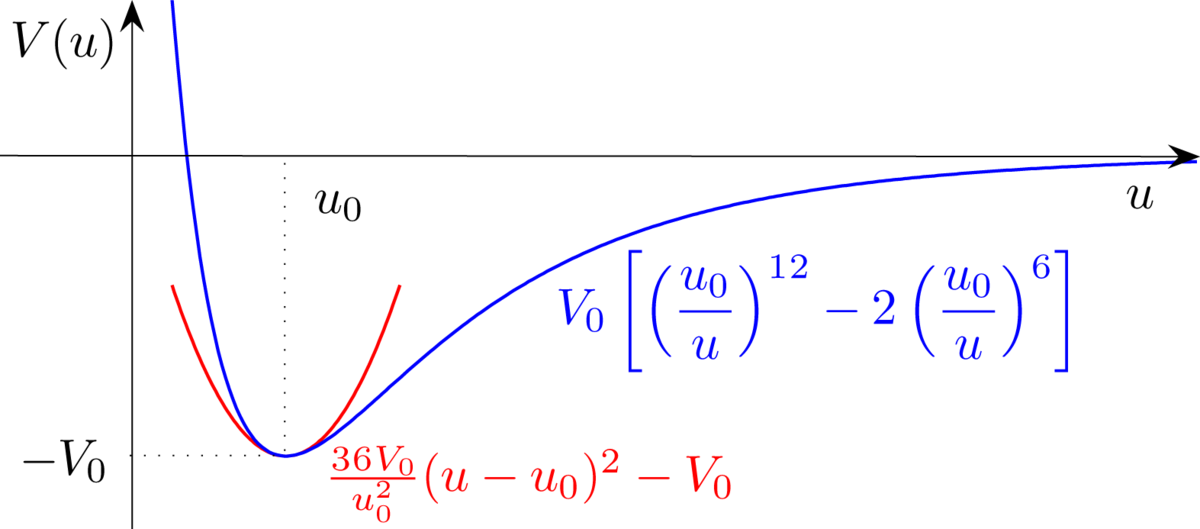
\includegraphics[width=0.9\columnwidth]{images/theory1.png}
		\caption{Harmonic Approximation for Lattice
		Dynamics}
		\label{fig:theory1}
	\end{figure}

	\begin{figure}[h]
		\centering
		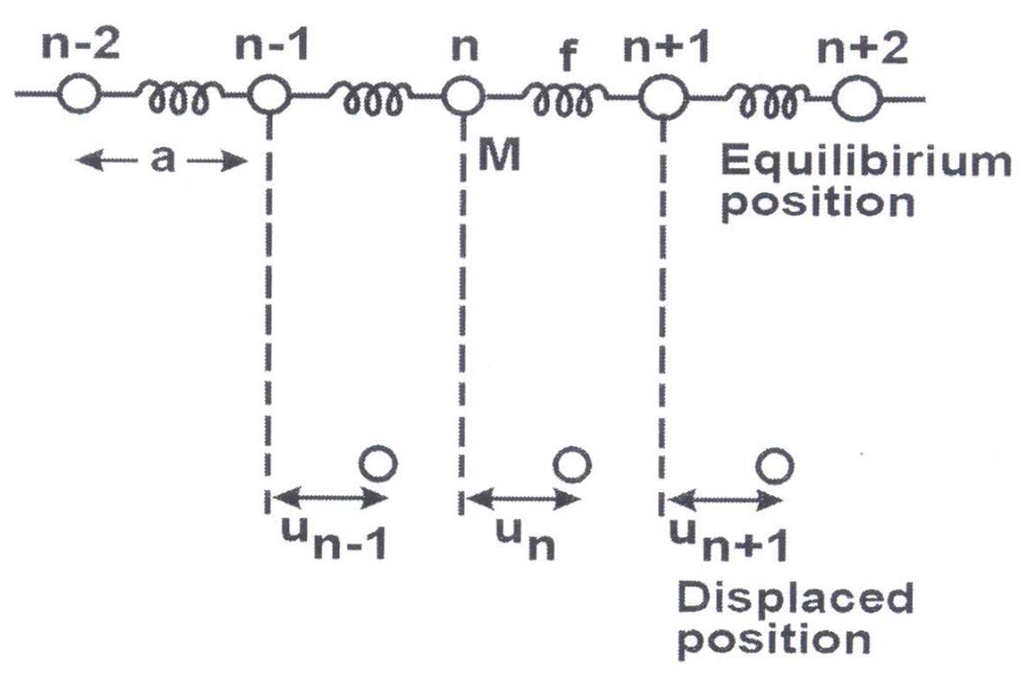
\includegraphics[width=0.9\columnwidth]{images/theory2.png}
		\caption{Spring Mass model of One Dimentional Linear Mono-atomic Lattice}
		\label{fig:theory2}
	\end{figure}

	\subsection{Monatomic Lattice Vibrrations}

		The harmonic approximation for a monoatomic crystal lattice is shown in \hyperref[fig:theory2]{Figure 2}. In \hyperref[fig:theory2]{Figure 2} these are the relevant constants:
		\begin{itemize}
			\item \textbf{a} $\rightarrow$ Lattice Constant
			\item \textbf{f} $\rightarrow$ Force constant
			\item \textbf{M} $\rightarrow$ Mass of the atom
		\end{itemize}

		On applying Newton's second law of motion and Hook's law for the sprin-mass system, we get the differential equation for the $n^{th}$ atom:

		\begin{equation}
			m \frac{d^2U_n}{dt^2} = f(U_{n+1} - 2U_n + U_{n-1})
			\label{eqn:1}
		\end{equation}

		where f corresponds to the force constant and $U_n$ is the displacement of the $n^{th}$ atom. Similarly, for $N$ number of particles at equilibrium particle distance $r$, there will $n$ coupled differential equations. Resonance would occur for the relation between length of the atomic chain in one dimension $(L = (N+1)r)$ and the wavelength of vibration, for an integer $m$ given as $2L = m\lambda$.
		
		Now, let us assume that the solution be of the form $U_n = A \exp(kx_n-\omega t)$. Substituting this in the differential equation with the boundary conditions of $x_N = x_0 = 0$, we get the following equation:

		$$\omega = \sqrt{\frac{4f}{m}}\abs{\;\sin\frac{ka}{2}}$$

		This is the dispersion relation, with $k$ denoting the $\sfrac{wavenumber}{wavevector}$. The Brilluoin zone for the newest (the independent values of $k$, values for which are indentical to other zones in the lattice) is supplied by the sin term as:

		$$\frac{-\pi}{a}\leq k \leq \frac{\pi}{a}$$

		The electronic circuit that is an equivalent for these monoatomic vibration is that on an LC low pass filter as shown in figure, the output voltage of which is measured around the capacitor.

		On solving for the current arcoss the n-th capacitor, we find a differntial equation similar to that of \hyperref[eqn:1]{Equation 1} given as:

		$$C\frac{d^2V_n}{dt^2} = \frac{1}{L}(V_{n+1} - 2V_n + V_{n-1})$$

		where capacitance $C$ is equivalent to the mass, inductance $L$ to $\sfrac{1}{force constant}$, and $V_i$ is the voltage across the $i^{th}$ capacitor. Similar solution leads us to